\chapter{Converting Theory to Experiment}
Eventhough, the method seems to have nice implications in theory, it is still way to early to celebrate. There is still a long way, before it can be used in the lab. In the this chapter, we will cover which differences there is between, what we see in our simulations and the actual measurements in the laboratory. This will place us in a position to perform the probable approximations and conversersions to make our method work in the lab:

\newthought{This is just a list of litterature and observations which we need to use for writing this chapter.}
\begin{itemize}
    \item In \cite{ikonen_qubit_2019} it seems like they just match the axis variable.  
\end{itemize}

\begin{figure}
    \centering
    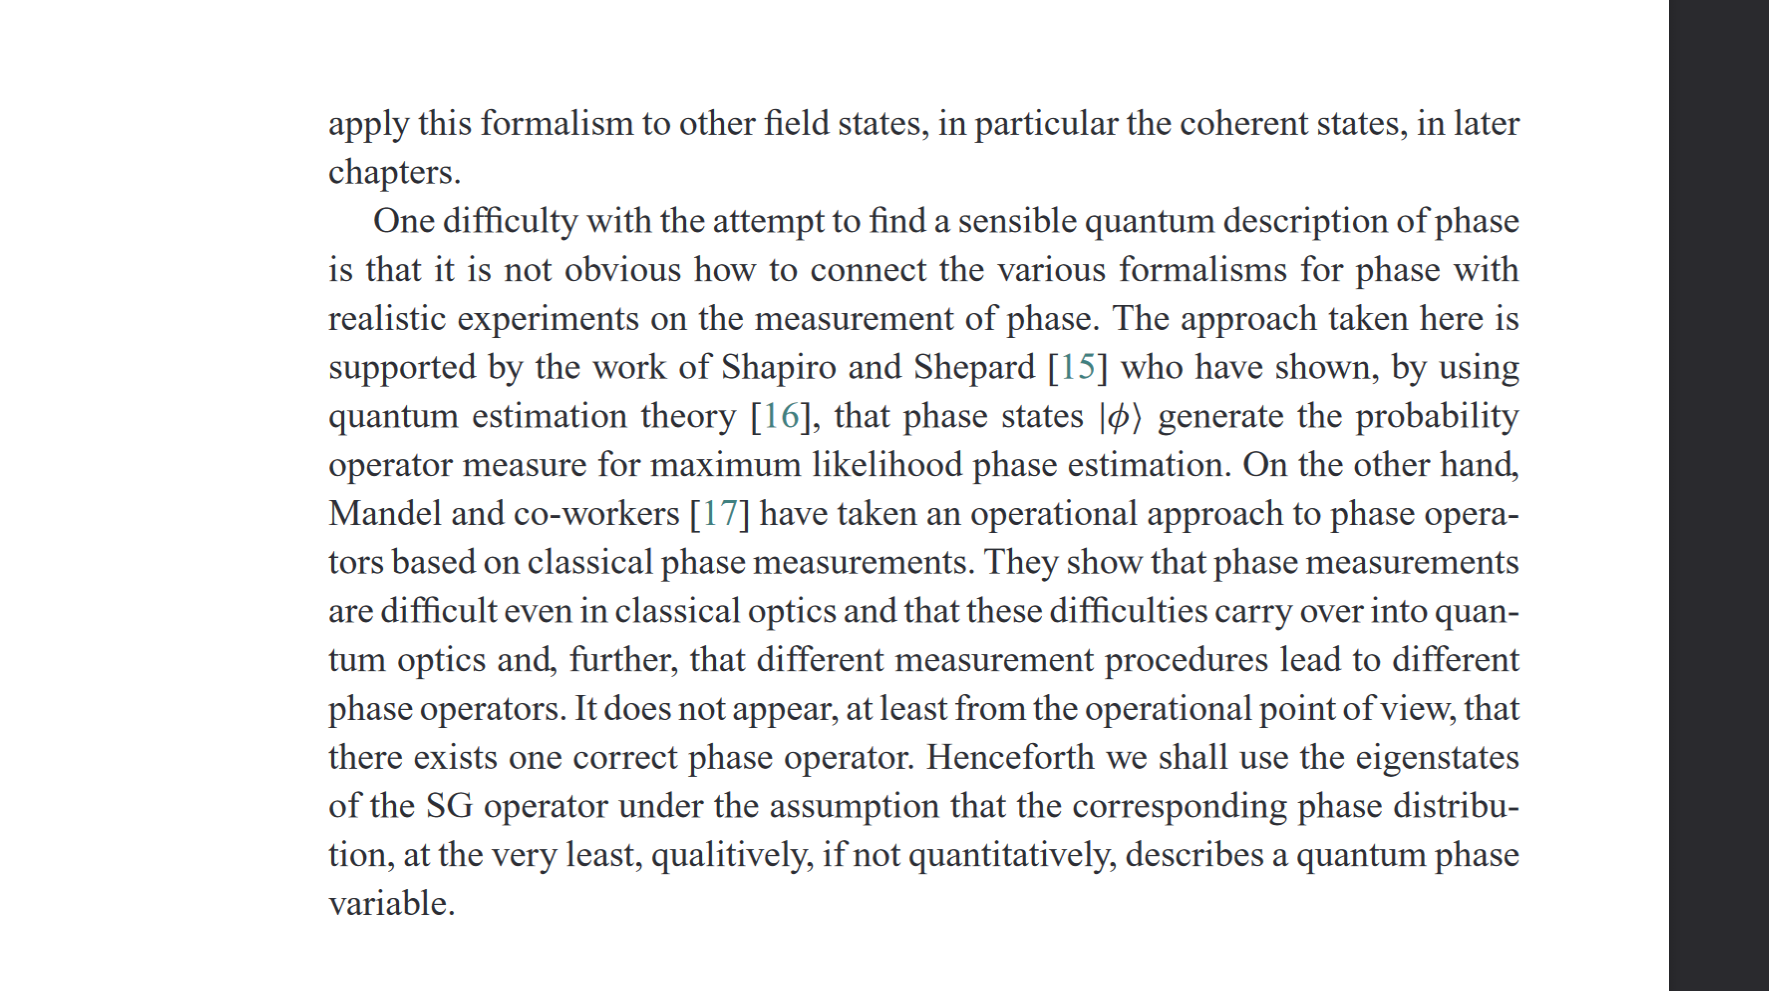
\includegraphics{Figs/insert_from_quantum_optics.png}
    \caption{Caption}
    \label{fig:my_label}
\end{figure}